\documentclass[letterpaper,11pt]{article}

%packages
\usepackage{amsfonts}
\usepackage{graphicx}
\usepackage[left=2cm,top=2cm,right=2cm,bottom=1.5cm,head=.5cm,foot=.5cm]{geometry}
\usepackage{url}
\usepackage{multirow}
\usepackage{longtable}
\usepackage{subfig}
\usepackage{float}
\usepackage{setspace}
\usepackage{lineno}
\usepackage{natbib}
\usepackage{amsmath}
\usepackage{authblk}
\usepackage{xr}
\usepackage{relsize}
\usepackage{tikz}
\usepackage{hyperref}

%new commands and so on
\providecommand{\keywords}[1]
{
  \small	
  \textbf{\textit{Keywords---}} #1
}

\DeclareMathOperator{\E}{\mathbb{E}}% expected value
\DeclareMathOperator{\var}{var}
\DeclareMathOperator{\cov}{cov}
\DeclareMathOperator{\cor}{cor}
\DeclareMathOperator{\mean}{mean}
\DeclareMathOperator{\se}{se}
\DeclareMathOperator{\sd}{sd}
\DeclareMathOperator{\prob}{P}

%attempt 1 at nat and sharp
%\newcommand{\nat}{\mathlarger{\natural}}
%\newcommand{\shp}{\mathlarger{\sharp}}

%attempt 2 at nat and sharp
%\newcommand{\nat}{\raisebox{1pt}{\mathsmaller{\mathsmaller{/\hspace{-2pt}/}}}}
%\newcommand{\shp}{\#}

%attempt 3 at nat and sharp
\newcommand{\nat}{%
\text{\hspace{-1.5pt}
\begin{tikzpicture}[scale=1.8]%
\draw (.333ex,0) -- (.333ex,1ex);%
\draw (.666ex,0) -- (.666ex,1ex);
\end{tikzpicture}%
}}
\newcommand{\shp}{%
\text{\hspace{-1.5pt}
\begin{tikzpicture}[scale=1.8]%
\draw (0,.333ex) -- (1ex,.333ex);%
\draw (0,.666ex) -- (1ex,.666ex);%
\draw (.333ex,0) -- (.333ex,1ex);%
\draw (.666ex,0) -- (.666ex,1ex);
\end{tikzpicture}%
}}
\newcommand{\test}{%
\text{
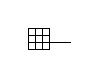
\begin{tikzpicture}[scale=1.8]%
\draw (0,0) -- (1ex,0ex);
\draw (0,0) -- (0ex,1ex);
\draw (0,1ex) -- (1ex,1ex);
\draw (1ex,0) -- (1ex,1ex);
\draw (0,.333ex) -- (2ex,.333ex);%
\draw (0,.666ex) -- (1ex,.666ex);%
\draw (.333ex,0) -- (.333ex,1ex);%
\draw (.666ex,0) -- (.666ex,1ex);
\end{tikzpicture}%
}}

\newcommand{\olr}{\overline{r}}
\newcommand{\olrs}{\overline{r}^{\shp}}
\newcommand{\olrn}{\overline{r}^{\nat}}
\newcommand{\bs}{\backslash}

%header material for paper
\title{Responses to referees for ``Asymmetric relationships and their effects on coexistence''}
\date{July 2023}

\begin{document}

\noindent \emph{Dear Editors,} \\

\noindent \emph{Thank you for the useful and very positive reviews of our manuscript, and for
the opportunity to resubmit a revised version. We have addressed all referee comments below and in
the manuscript, and hope the paper can now be rapidly accepted. } \\

\noindent \emph{We have replied to referee comments below in italic, with each response preceded
by ``***'', to make our responses easier to find.} \\

\noindent \emph{We submit the following pdf files: ...} \\

\noindent \emph{We additionally submit the following latex files, necessary for compiling the
main text latex: ...} \\

\noindent \emph{The document showing the changes we made does not include links such as citations and
references to figures, but it does accurately represent the changes made to the text. 
If all latex files are deposited into the same folder, it should then be possible to 
compile the main text latex from that folder.} \\

\noindent \emph{We again thank the referees and editors for their feedback and positive reviews!} \\

\noindent \emph{Yours,}

\noindent \emph{Dan Reuman and Jasmin Albert} \\

\noindent \textbf{Comments of referee 1:} \\

%The C) that precedes each comment is because we will later add numbers, C1, C2, etc., after making sure these
%comments are divided up to our liking. Then we can refer to each comment by its number, which can be useful.
\noindent C1) This is a very interesting paper that adds to our understanding of modern coexistence theory through the decomposition of the ways in which competitive pressure and environment can be correlated.\\

\noindent ***\emph{Thank you for the positive feedback!} \\

\noindent C2) Specifically, the focus is on asymmetric tail association (ATA), by which two random variables with given, fixed marginal distributions and correlation can nevertheless differ in the way that their right and left tails are correlated. This is one among many ways that one could characterize or decompose the full bivariate distribution between competition and environment, but the authors argue and demonstrate that ATAs of this kind are (a) prevalent in natural systems and (b) can have a meaningful and sometimes qualitative effect on the outcome of coexistence between two species.  The combination of results for theoretical distirbutions but also for experimental data is very powerful and convincing. \\

\noindent ***\emph{Thank you for the positive feedback!} \\

\noindent C3) I have one overarching question, which I think may be important for ensuring that those points (a) and (b) are robust and then some minor comments that may improve the readability of the manuscript for the EL audience. \\

\noindent ***\emph{response} \\

\noindent C4) My biggest question is related to the removal of ATAs from a given true bivariate distribution.  This is described in SI Section S2 and shown visually for an example in SI Figure S1. 

My first comment related to this is that some form of this text (whcih is relatively short---around half a page in the SI) and, importantly, the Figure should be in the main text.  I think this is such a key part of the definitions that are being used for the rest of the paper that readers will want to get an intuition for what the "partial sharp" distributions look like and how they are arrived at. \\

\noindent ***\emph{<Move SI Fig S1 and associated text back to the MT – at least two referees asked for it.>} \\

\noindent C5) Perhaps equally important to clarifying this process for the readership is whether this process is unique. I could not quite get a sense of whether there could be alternative versions of this removal of ATA from a bivariate distribution, that still satisfy the authors' constraints on marginal distributions and overall correlation between the two variables. Are there alternatives, or is the authors' procedure unique in achieving the desired outcome?  If the former, then I would want to understand if the outcomes downstream tend to be robust to the specific method used. If the latter, it would be helpful to have an explanation as to why this is a unique decomposition. \\

\noindent ***\emph{<Address the issue of whether and to what extent the process of removing ATAs is unique – probably just with a one-sentence callout in the main text, and some material in the SM (possibly a new section)>} \\

\noindent C6) The notation by which the partial sharp variables are introduced was a little unintuitive to me.  For example, when the authors compare the expectation values 
$E[r(E,C)]$ and $E[r(E^{||},C^{||})]$, what is really changing is the distribution over which the expectation values are evaluated.  Maybe this is standard notation, but somehow it may be clearer to put the subscript on the E for expectation value, to indicate that the probability distribution used to generate the definition of the averaging is what differs between the two expressions, while the variables E and C themselves are in the end just dummy variables to be integrated over.  \\

\noindent ***\emph{<This one asks for possibly changing notation. I don’t think we should do it, but we need to explain in a response what is actually going on, why we chose the notation that we do, and then add a new SM section addressing what the referee is talking about. Actually it’s the bivariate distribution that changes when you apply ||, tho the marginals are not changed. So the referee does have a bit of a point – E^{||} by itself is actually the same distribution as E, it’s just that it’s a different random variable in the sense of being related differently to C^{||} than E is to C. This is the same issue with the # notation that has already been established. It’s actually formally correct in the sense of random variables if we view *all* our random variables as being measurable functions from the *same* probability space. So in the end the referee does not really have a point if one wants to be formal. But you can explain all this in a new sup mat section.>} \\

\noindent C) It was not clear to me what the reasoning was for including the correlation and ATAs in abundance for the two planktonic species in Figure 1(d) and (e).  These ATAs in abundances don't in an obvious (to me) way translate into ATAs of the underlying environment and competition variables for each species. Is this really a demonstration that ATAs occur for C and E?  If not, then it seems to be like saying ATAs exist somewhere in nature, and therefore might be present in our focal situation, which is not such a very strong reason to show (d) and (e).  Maybe I am missing something. \\

\noindent ***\emph{<Yes, the referee is right about this, that's what we're doing. Just admit to it and justify doing it anyway because a) we were asked to include this kinda thing by poeple who read it before we submitted; b) the value is not only in showing that ATAs occur, but also in helping people understand more fully what they look like; and c) we cannot show ATAs in E and C (at least not this early in the paper), becuase no one has looked at this before so there is no prior evidence of it.>} \\

\noindent C) The authors mention that $r_{i \bs i}$ indicates growth rate of species when $i$ is rare and $j$ is at steady state.  I think $r_{j \bs i}$ must also assume that $j$ is at steady state, but this isn't mentioned. Perhaps that could be added for completeness. \\

\noindent ***\emph{<Just do this and say we did it - it's a good enough idea.>} \\

\noindent C) E.g. line 100 needs removal of the word "are" or the addition of the word "and" somewhere to make sense. I'd consider going through the paper carefully for any typos or small corrections of this kind. \\

\noindent ***\emph{response} \\

\noindent \textbf{Comments of referee 2:} \\

\noindent C) In their paper the authors decompose the “storage effect” into two separate effects, what they call the “asymmetric tail association” and the covariance term per se. The authors explain well why they do this and why they think this may be important. Additionally, they show the best possible efforts to convince the readers why such a decomposition may be important and what we may learn from it. Overall, the paper is interesting and quite understandable. I think the authors have done a very good job. \\

\noindent ***\emph{Thank you for the very positive feedback!} \\

\noindent C) Unfortunately, I’m personally not convinced that storage effect (and therefore probably ATA) are relevant for coexistence in nature and therefore I’m sceptical about this new approach. I want to be clear that this is, in part, my personal opinion and I know experts in the field which have a very different view. What the authors have shown (and it appears to be correct) is that in a model where niche differentiation via different resources and predators is impossible, then ATA can be an important driver of coexistence, and I agree. However, in every application where both storage effect, relative non-linearity and niche differentiation have been measured, there we see that storage effect and relative non-linearity where very small compared to simple resource differentiation. But, one might argue, that we have barely any such empirical applications, and I would agree, which is why I label this my personal opinion. (The few papers that I know of are \href{https://nam10.safelinks.protection.outlook.com/?url=https%3A%2F%2Fdoi.org%2F10.1002%2Fecy.2726&data=05%7C01%7Cd294r143%40ku.edu%7C13ab816eaf2a49c27ea808db784a67cf%7C3c176536afe643f5b96636feabbe3c1a%7C0%7C0%7C638236033192197676%7CUnknown%7CTWFpbGZsb3d8eyJWIjoiMC4wLjAwMDAiLCJQIjoiV2luMzIiLCJBTiI6Ik1haWwiLCJXVCI6Mn0%3D%7C3000%7C%7C%7C&sdata=HbUTjzCNQrvGSARY5u3Eqme88DbKiNyiAVNOUGzjcbE%3D&reserved=0}{Zepeda et al. 2019, Ecology}, \href{https://nam10.safelinks.protection.outlook.com/?url=https%3A%2F%2Fdoi.org%2F10.1890%2F14-1741.1&data=05%7C01%7Cd294r143%40ku.edu%7C13ab816eaf2a49c27ea808db784a67cf%7C3c176536afe643f5b96636feabbe3c1a%7C0%7C0%7C638236033192197676%7CUnknown%7CTWFpbGZsb3d8eyJWIjoiMC4wLjAwMDAiLCJQIjoiV2luMzIiLCJBTiI6Ik1haWwiLCJXVCI6Mn0%3D%7C3000%7C%7C%7C&sdata=KKIBuLjBN2vNGWfEpduAGGrMAt7ov9a4F53CmlZQlO0%3D&reserved=0}{Chu and Adler 2015}, and Ellner et al. 2019, see also the new paper by \href{https://nam10.safelinks.protection.outlook.com/?url=https%3A%2F%2Fesajournals.onlinelibrary.wiley.com%2Fdoi%2Fepdf%2F10.1002%2Fecm.1585&data=05%7C01%7Cd294r143%40ku.edu%7C13ab816eaf2a49c27ea808db784a67cf%7C3c176536afe643f5b96636feabbe3c1a%7C0%7C0%7C638236033192197676%7CUnknown%7CTWFpbGZsb3d8eyJWIjoiMC4wLjAwMDAiLCJQIjoiV2luMzIiLCJBTiI6Ik1haWwiLCJXVCI6Mn0%3D%7C3000%7C%7C%7C&sdata=YaqsZ6axu6rYV12kh9IiRIbES7ZUMWIN7HXgB08iPzc%3D&reserved=0}{Stump and Vasseur}, which I have not yet read fully) In my understanding, ATA is a decomposition of storage effect into even more components, therefore I would expect, on average the ATA effect to be slightly smaller than storage effect (but, as you have shown can also be larger than storage effect). I would therefore assume that ATA is generally weak compared to niche differentiation (but again, admittedly based on few datapoints). Obviously, the authors may disagree with my personal view, in this case I’d like to see a discussion of this. \\

\noindent ***\emph{<Add a discussion, either in the Discussion or in an SM section called something like 
``Additional discussion point". Acknowledge the viewpoint, state that insufficient studies have been done to be sure
. 2) >} \\

\noindent C) I like the conceptual idea of removing the long tail. \\

\noindent ***\emph{response} \\

\noindent C) However, I have somewhat difficulties to precisely understand/be sure I correctly understood what this does. I suggest you move a simpler version of Fig S1 into the main text and show the actual distribution, the uncorrelated distribution of $E$ and $C$, but same marginal distribution, and the distribution with the same covariance, but the ATA removed. Additionally, it might be beneficial to indicate which distribution is then used to compute which part of the decomposition. For example, in Figure S1 d you show $E_i^{||}$, but from my understanding this distribution would be used to compute $E_i^{(EC)}$, correct? \\

\noindent ***\emph{response} \\

\noindent C) You focus solely on storage effect with the argument that it’s the only where ATA can actually occur. But on a broader level you essentially decompose the EC distribution into it’s different momentums. One only carrying about the mean (i.e. first order correct), one with only carrying about the mean and covariance (i.e. getting the first two orders correct), and one with all other orders correct. Given this interpretation of your work, I might apply the same logic to the relative-nonlinearity, where I decompose the relative non-linearity into the variance term and the term with long tails. (one might also even decompose the actual distribution into more distributions, getting successively more and more momentums of the distribution correct, but I would argue that this is probably less useful). \\

\noindent ***\emph{response} \\

\noindent C) L34: I found this sentence confusing due to the two “betweens” and it’s not immediately clear to what they “bound” \\

\noindent ***\emph{response} \\

\noindent C) L41: The “we” is slightly confusing because the author teams share only one author \\

\noindent ***\emph{response} \\

\noindent C) L48: I do not know these on the top of my head, and likely many other readers will neither, so maybe quickly refresh our memory \\

\noindent ***\emph{response} \\

\noindent C) L49: This is not immediately clear to me why (obviously, you’ve shown this in the other paper). Is it possible to briefly state why? \\

\noindent ***\emph{response} \\

\noindent C) L61: What if not? Or many readers have only rough understanding of it, maybe quickly refresh or refer to later \\

\noindent ***\emph{response} \\

\noindent C) Sidenote: After writing these few comments it appears to me that you seem to have a very knowledgeable reader in mind, which may not be the case for a general journal as Ecology letters. \\

\noindent ***\emph{response} \\

\noindent C) L64: Narwani 2013 is actually not a good reference because it did not include any temporal variation, a better one would be Letten et al. 2019 in PNAS. \\

\noindent ***\emph{response} \\

\noindent C) L74: The optimum might actually be the same, but they need different responses Eq. 1: I would not use any equations in the introduction, and in general this part of the introduction did not feel like an introduction at all and might require a different sub-section \\

\noindent ***\emph{response} \\

\noindent C) L93: I suggest ``Note that $N = N_1(t) + N_2(T)$ is constant through time''. \\

\noindent ***\emph{response} \\

\noindent C) L95-99: I think this is a great teaser to get the readers to later dive in into your mathematics \\

\noindent ***\emph{response} \\

\noindent C) L126: Do you do this in the appendix? \\

\noindent ***\emph{response} \\

\noindent C) Eq 2.: I thought we also have to remove the effect of C varying alone and E varying alone? Is this included in the $\#$ term automatically? \\

\noindent ***\emph{response} \\

\noindent C) Eq. 6: Maybe highlight that you use different brackets ([EC] versus (EC)), or probably even better, make 5 and 6 one equation using curly under brackets. \\

\noindent ***\emph{response} \\

\noindent C) L230 $\mu_1-\mu_2$ is negative, why not take $\mu_2-\mu_1$? \\

\noindent ***\emph{response} \\

\noindent C) L316: So why do you show values of $\sigma >6$? And also maybe highlight this in the figure Figure 1d and e: I’m semi convinced by these distributions showing ATA. In 1d it simply appears that the variance scales with the density. 1e is quite unconvincing to me. That’s generally fine, but figure 1 seems to be a conceptual figure, so I wonder whether you don’t have a better example? \\

\noindent ***\emph{response} \\

\noindent C) Figure 2: I recommend to add a line at $y = 0$. Also the different subgraphs have different $y$-scales which I’m not sure is beneficial, but unsure myself. \\

\noindent ***\emph{response} \\

\noindent C) Figure 2 and 3: It appears that ATA is almost never the relevant factor, however I wonder whether this is because ATA is relatively weak, or whether the same analysis of say $\delta_i$ would lead to a similar pattern, it might be worth creating these graphs in the appendix to strengthen your case. \\

\noindent ***\emph{response} \\

\noindent C) Figure 2: ATA is always positive, so how can it lead to ATA exclusion? (or ATA rescue in case I misunderstood). \\

\noindent ***\emph{response} \\


\noindent \textbf{Comments of referee 3:} \\

\noindent C) This is a well performed paper pointing out that asymmetric tail associations (ATA) in a correlation between the environment and competition can be an important mechanisms of coexistence previously overlooked. ATAs can give additional mechanisms that either promote or hinder coexistence in a similar fashion and magnitude to other previously recognised mechanisms such as the storage effect. To illustrate these ideas the authors combine results from mathematical models, simulations, and empirical examples, and show that under a certain combination of parameters ATAs can be a significant mechanism of species coexistence. \\

\noindent ***\emph{response} \\

\noindent C) Overall, I agree with the authors that the role of ATAs in coexistence has not been properly considered and the manuscript give convincing results of the importance of ATAs. \\

\noindent ***\emph{response} \\

\noindent C) However in order to reach a broad audience of ecologists, the manuscript needs to reach a balance between mathematical definitions and simple explanations. Otherwise, it can remain to technical and of little importance to ecologists interested in the role of environmental variability of community dynamics. I will give some examples where the message can be improved, but I would suggest the authors to do the same effort themselves in other parts of the manuscript. \\

\noindent ***\emph{response} \\

\noindent C) At the beginning of the introduction the authors cite previous work to show the prevalence and importance of ATAs for population dynamics, and the stability of ecological communities, and Fig.1 illustrate what ATAs mean in a clear example, yet it is not well explained or at least it was not clear to me how ATA can either promote or hinder coexistence in these initial sentences. \\

\noindent ***\emph{response} \\

\noindent C) Then the explanation of the importance of ATAs is done in relationship with the explanation of the storage effect. In detail, the explanation of the storage effect is superb, but how ATAs enter in play is not well solved. It is just mentioned that ATAs can modify the EC covariation, which I believe is not enough, a reader might not understand later the explanation when the lottery model is presented. \\

\noindent ***\emph{response} \\

\noindent C) ATAs can not only modify the importance of the storage effect but also of other mechanisms such as relative non-linearity, which is based on how competition fluctuates in ways that favor the competitor. Could the authors briefly indicate how this could occur? \\

\noindent ***\emph{response} \\

\noindent C) The lottery model is used to illustrate the importance of ATAs, and two types of fecundities are taken into account (log-normal and beta), can the author explain why both are important, and later on the results and discussion why ATAs play a major role with beta fecundities and not with log-normal \\

\noindent ***\emph{response} \\

\noindent C) The model used for the chemostat is in its formulation quite different compared to the lottery model. Although the technical details are left for the supplementary material, can the authors explain more in the detail in the main text how the importance of ATAs can be used for this particular model. \\

\noindent ***\emph{response} \\

\noindent C) The chemostat model is parameterized with information from a previous study, but does this model reproduce observed dynamics of the diatom system? this needs to be shown otherwise the importance of ATAs will be considered for another dynamics that do not correspond to the observed ones. \\

\noindent ***\emph{response} \\


\noindent \textbf{Comments of the editor:} \\

\noindent C) This study novelty is the focus on assymetric tail association between competition and environmental conditions as a mechanism of coexistence. \\

\noindent ***\emph{response} \\

\noindent C) The manuscript is very theoretical with a highly technical language hard to follow by a broad range of ecologists. My main suggestion is that the authors need to rewrite it in several parts to make it accessible and convincing. The authors have to make an effort to use a more biological/ecological language with reference to real world potential examples/cases/systems. Some mathematical material could be moved to Supplementary material. \\

\noindent ***\emph{response} \\

\end{document}